\documentclass{ximera}

\input{preamble.tex}

\author{Gregory Hartman \and Matthew Carr}
\license{Creative Commons 3.0 By-NC}
\acknowledgement{https://github.com/APEXCalculus}

\begin{document}
\begin{exercise}

\outcome{Identify when a limit does not exist.}
\outcome{Calculate limits of piecewise functions.}

\tag{limit} 
\tag{piecewise} 
\tag{discontinuous}

%% BADBAD DNE answer
  Find 
  \[
  \lim_{x\to 2} f(x)
  \begin{prompt}
  = \answer{DNE}.
  \end{prompt}
  \]
  where
  \[
  f(x) = \begin{cases}
    x+2 & x\leq 2, \\
    3x-5 & x>2.
  \end{cases}
  \]
    \begin{hint}
     Both pieces of $f(x)$, $x+2$, for $x\le2$, and $3x-5$, for $x>2$,
     are continuous for all $x$. However, for the limit
     $\lim_{x\to2}f(x)$ to exist, both the left-hand and the
     right-hand limits of $f(x)$ at $2$ must exist and be equal.
    \end{hint}
     \begin{hint}
    	Take a look at the graph of the function
    \begin{center}
     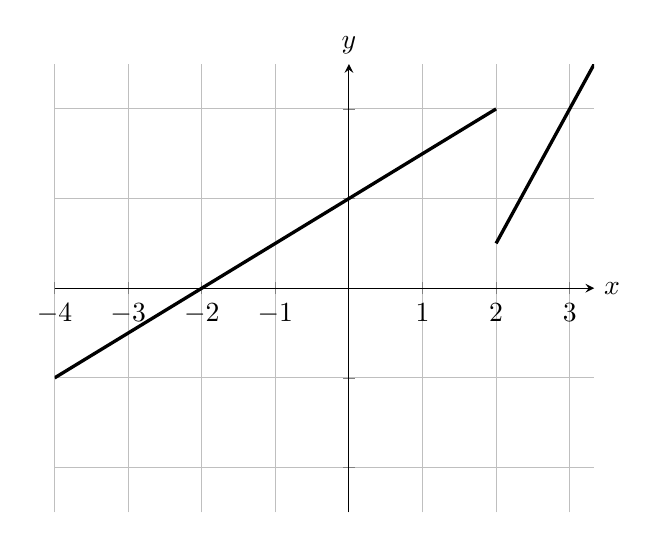
\begin{tikzpicture}
	\begin{axis}
	[ymin=-5,ymax=5, axis lines=center,xlabel=$x$,ylabel=$y$,every axis y 
	label/.style={at=(current axis.above origin),anchor=south},every axis x label/.style={at=(current axis.right of origin),anchor=west},
	domain=-4:4,
	yticklabels={},
	ymajorgrids=true,
	grid = major
	]
	\addplot[domain=-4:2,very thick,smooth]
	{2+\x};
	\addplot[domain=2:4,very thick,smooth]
	{3*\x-5};
	\end{axis}
       \end{tikzpicture}      
      \end{center} 
    \end{hint}
    \begin{hint}
     Evaluating $\lim_{x\to2^{+}}f(x)$ we see that it is equal to
     $1$. This follows because, for $x>2$, we are on the piece of
     $f(x)$ given by $3x-5$ and the limit
     $\lim_{x\to2}\left({3x-5}\right)=3\cdot\lim_{x\to
       2}(x)-\lim_{x\to2}\left({5}\right)=1$, certainly. On the other
     hand, evaluating $\lim_{x\to2^{-}}f(x)$ we see it is equal to
     $4$. This follows because, for $x\le2$, we are on the piece of
     $f(x)$ given by $x+2$ and the limit
     $\lim_{x\to2}\left({x+2}\right)=\lim_{x\to2}(x)+\lim_{x\to2}\left({2}\right)=4$,
     certainly. These are not equal, so $\lim_{x\to 2}f(x)$ does not
     exist.
    \end{hint} 
\end{exercise}

\end{document}
